\documentclass[12pt,a4paper,twoside]{article}
\usepackage[UKenglish]{isodate}
\usepackage[pdfborder={0 0 0}]{hyperref}
\usepackage[margin=25mm]{geometry}
\usepackage{graphicx}
\usepackage{parskip}
\usepackage{enumitem}
\usepackage{microtype}
\usepackage{float} % for figures 'n' stuff
\usepackage{graphicx} % for pictures
\usepackage{longtable} % so we can break the timetable across two pages

\usepackage[style=numeric,backend=bibtex]{biblatex}
\bibliography{refs.bib}

\begin{document}

\cleanlookdateon

\begin{center}
\Large
Computer Science Tripos -- Part II -- Progress Report\\[4mm]
\LARGE
A Comparison of Statistical Models and Recurrent Neural Networks for the
Generation of Music\\[4mm]

\large
Alex Coplan (\texttt{ajc310}), St Catharine's College


\today
\end{center}

\vspace{5mm}

\textbf{Project Supervisor:} Matthew Ireland (mti20)

\textbf{Director of Studies:} Dr S. Taraskin (snt1000)

\textbf{Project Overseers:} Prof.\ M. Fiore \& Prof.\ I. Leslie\\

\textit{The goal of this project is to implement and compare two algorithms for
melody generation. In particular, the project compares the performance of
Recurrent Neural Networks with that of Multiple Viewpoint Systems (ensembles of
higher-order Markov chains) on this task.}

\section*{Work Complete to Date}

\subsection*{Multiple Viewpoint Systems}

A multiple viewpoint system (MVS) meeting the success criteria outlined in the
proposal has been implemented, along with accompanying unit tests. The specific
functionality implemented is as follows:
\begin{itemize}
  \item At a high level, a general framework has been established (using C++
    templates) for implementing context models, viewpoints, and multiple
    viewpoint systems.
  \item A representation of musical events has been developed: in particular,
    for the space of musical events in a set of Lutheran chorale melodies.
  \item Context models, providing the underlying predictive functionality of
    viewpoints, have been implemented. These may be of arbitrary order (at
    runtime) and parameterised on arbitrary events (at compile time, using
    templates). 
    \begin{itemize}
      \item Context models output \emph{distribution objects} as their
        predictions. A weighted entropy scheme has been implemented for
        combining such distributions. 
      \item Context models can evaluate the cross-entropy of input sequences of
        events against their predictions.
    \end{itemize}
  \item A general abstraction around viewpoints has been implemented, and the
    following musical viewpoints have been implemented: \emph{pitch},
    \emph{seqint} (sequential melodic interval), \emph{duration}, \emph{rest}.

  \item A wrapper around the high quality pseudo-random number generator
    \texttt{xoroshiro128+} was written for use with the C++11 \texttt{<random>}
    library. This PRNG is used for sampling from MVSs.

\end{itemize}

\begin{figure}[H]
\centering
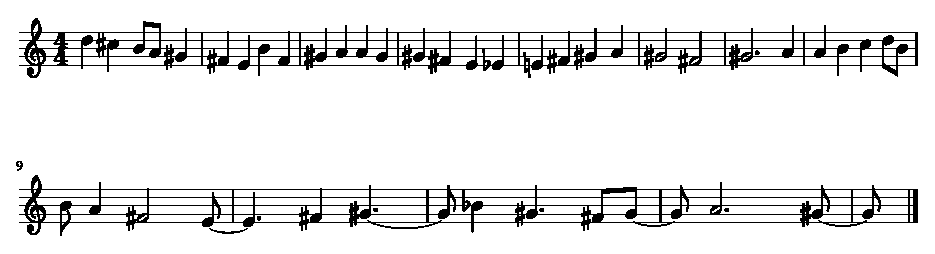
\includegraphics[width=400pt]{figs/mvs_trimmed.eps}
\caption{Sample from MVS generated by random walk.}
\label{fig:mvs-out}
\end{figure}

The output of the MVS is currently of lower quality than that of the RNN.
Considering the example in Figure~\ref{fig:mvs-out}, we see that, unlike the
RNN's output, there is no stable tonal centre (although E major is suggested)
and the composition is rhythmically weak. Viewpoints to fix these problems and
improve the overall performance of the MVS should be completed in the second
iteration.

\subsection*{Recurrent Neural Nets}

A Recurrent Neural Net (RNN) meeting the success criteria outlined in the
proposal has been implemented. The RNN was implemented in Python using Google's 
TensorFlow library, and makes use of long short-term memory cells. 

The original architecture has been modified to include an adaptation specifically
for generating music: the current position in the bar is given as input to the
network in addition to the musical event at the previous timestep. These input
\emph{clock neurons} help the network to learn to write music in a particular
time signature.

Various pre-processing steps to the corpus such as \emph{tonal inflation}
(inflation of training data by transposing music into multiple keys) lead to
improvements in the performance of the RNN.

\begin{figure}[H]
\centering
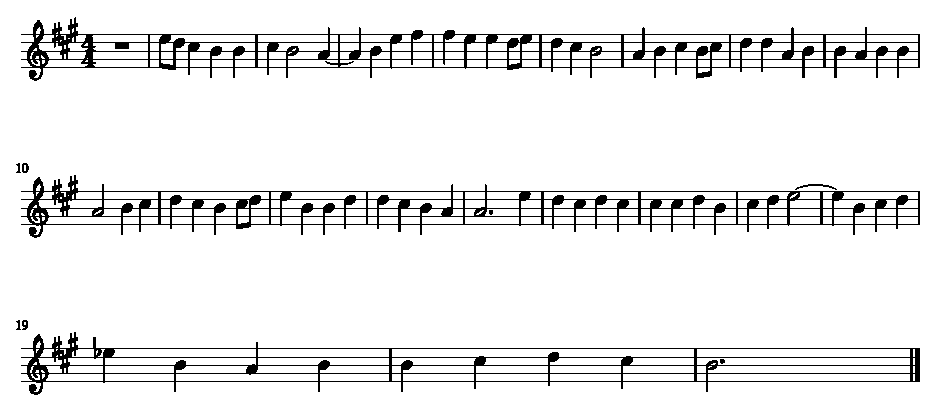
\includegraphics[width=400pt]{figs/rnn_trimmed.eps}
\caption{Sample from RNN generated by random walk.}
\label{fig:rnn-out}
\end{figure}
Figure~\ref{fig:rnn-out} demonstrates that the RNN has learned to compose music
with a stable tonal centre (in this case, A major). Note that random walk is a
poor sampling algorithm, since a noisy, low-probability decision can force the
algorithm to make a series of low-probability choices. This can be observed from
the third line in the above. I intend to implement a global sampling algorithm
to this end.

\subsection*{Other Milestones}

Ethics committee approval received.

\section*{Progress in relation to Timetable}

Currently the project is approximately two weeks behind schedule. Everything up
to this point in time has been completed except for the second iteration of the
MVS. This is due to the first iteration of the MVS taking longer than expected.
The second iteration of the RNN is complete. 

The first iteration of the MVS took until approximately 04/01/17, when the
second iteration was due to finish. RNN implementation started at this point,
and continued until 02/02/17.

\section*{Plan from Now}

It should now be possible to complete the second iteration of the MVS alongside
the evaluation preparation over the next two weeks. Sufficient slack in the
timetable was allowed for such an occurrence.

Preparation for the evaluation stage will be carried out in the form of
designing the survey questions that will be used and implementing a website to
facilitate this.

\end{document}
